\documentclass[aps, 12pt]{revtex4}
\usepackage[english]{babel}
\usepackage[utf8]{inputenc}
\usepackage[T1]{fontenc}
% \usepackage{NotesTeX}
\usepackage{subfigure}
\usepackage{tikz}
\usetikzlibrary{arrows}
\usepackage{multirow}
\usepackage{listings}
\usepackage{extarrows}
\usepackage{parskip}
\usepackage{eurosym}
\usepackage{footmisc}
\usepackage{kantlipsum}
\usepackage{algorithm}
\usepackage{algpseudocode}


\def\thesection{\arabic{section}}

\renewcommand{\deg}{^{\circ}}
\newcommand\numberthis{\addtocounter{equation}{1}\tag{\theequation}}
\newcommand{\hksqrt}[2][]{\ \mathpalette\DHLhksqrt{[#1]{#2\,}}}
\def\DHLhksqrt#1#2{\setbox0=\hbox{$#1\sqrt#2$}\dimen0=\ht0
    \advance\dimen0-0.3\ht0
    \setbox2=\hbox{\vrule height\ht0 depth -\dimen0}
    {\box0\lower0.65pt\box2}}

\graphicspath{{figs/}}
\newcommand{\includegraphicsmaybe}[2][]{\IfFileExists{../plots/#2}{\includegraphics[#1]{#2}}{\includegraphics[width=0.7\linewidth]{giffel.jpg}}}



\begin{document}

\author{Håkon Olav Torvik}
\title{\Huge Problem Set 3 \\ \small Math228B Numerical solutions to differential equations}
\affiliation{UC Berkeley}
\date{\today}


\maketitle

\section*{Problem 1}

\section*{Problem 2}
\subsection*{Part a}
For this part, I simply plug in the equation for the linear transfinite interpolation in the lecture slides, and use $x(\xi)=\xi$ to transform the unit-square into $\Omega$ with a linear mesh. The resulting mesh is shown in Figure \ref{fig:tfi_linear}.

\begin{figure}
    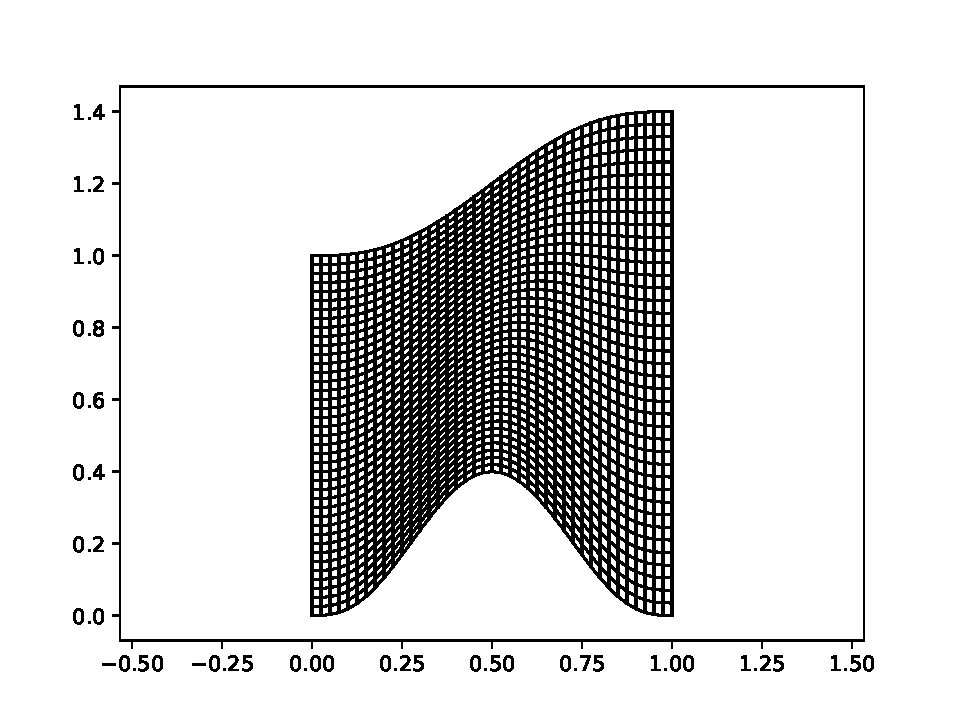
\includegraphics[width=0.8\linewidth]{linear.pdf}
    \caption{Linear transfinite interpolation of domain $\Omega$.}
    \label{fig:tfi_linear}
\end{figure}

\subsection*{Part b}
Using cubic Hermite interpolation gives more degrees of freedom, which can be used to specify the normal vector of the grid at the boundaries. Here $\partial R = T\hat{n}$ will be used at all the boundaries, where $\hat{n}$ is the unit normal vector in the positive $\xi$ and $\eta$ directions, and $T$ is a parameter. For $\xi = 0 \land \xi=1$, the boundary is straight, so $\hat{n}_{lr} = [1, 0]$.

The normal vector at the bottom I find by rotating the tangential vector by $\pi/2$, like so:
\begin{equation*}
    n_{bottom}(x) = \begin{pmatrix}
        -dy_{bottom}(x) \\
        dx
    \end{pmatrix} = \begin{pmatrix}
        -\partial_x (1+Ax^3(6x^2-15x+10)) \\ \partial_x x
    \end{pmatrix} = \begin{pmatrix}
        64\cdot 3Ax^2(1-x)^2(2x-1) \\ 1
    \end{pmatrix}.
\end{equation*}

Equivalently, at the top, it is
\begin{equation*}
    n_{top}(x) = \begin{pmatrix}
        -\partial_xy_{top}(x) \\ \partial_xx
    \end{pmatrix} = \begin{pmatrix}
        -3Ax^2(6x^2 - 15x + 10) - A*x^3(12x - 15) \\ 1
    \end{pmatrix}.
\end{equation*}

$x$ is no longer linear in $\xi$, so I use the Hermite polynomial to transform it, as
\begin{equation*}
    x(\xi) = H_0(\xi) + T\tilde{H}_0(\xi) + T\tilde{H}_1(\xi).
\end{equation*}

Now every thing is ready to be put together, and the grid is given by
\begin{equation*}
    \hat{R}(\xi, \eta) = H_0(\eta)E(\xi, 0) + H_1(\eta)R(\xi, 1) + \tilde{H}_0(\eta)R_{\eta}(\xi, 0) + \tilde{H}_1(\eta)R_{\eta}(\xi, 1)
\end{equation*}
The resulting transform from the unit square is shown in Figure \ref{fig:tfi_orth}.

\begin{figure}
    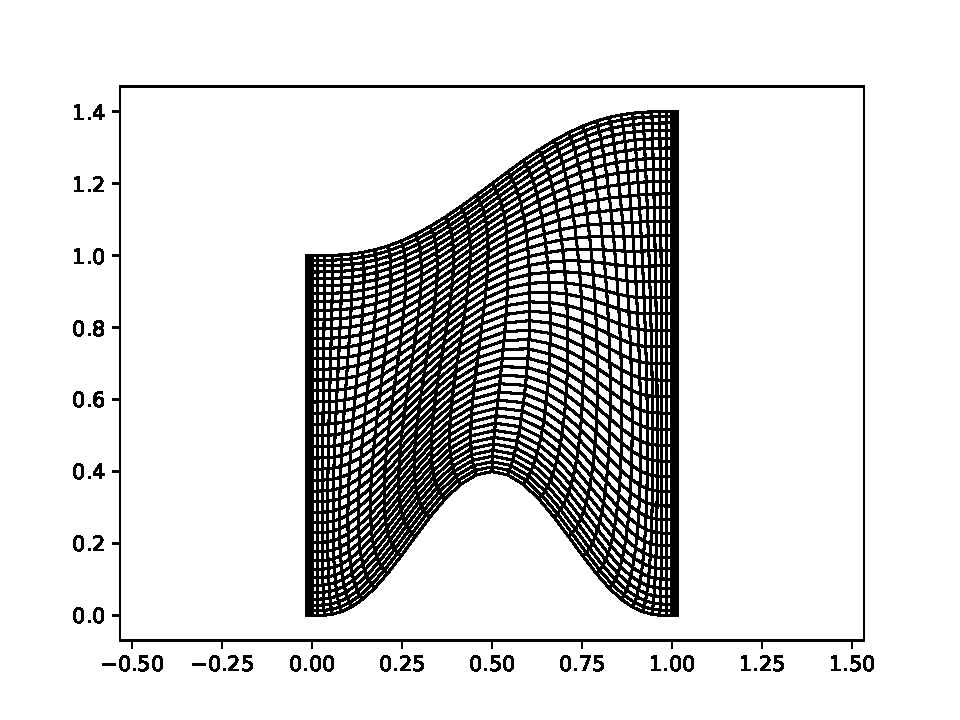
\includegraphics[width=0.8\linewidth]{orthogonal.pdf}
    \caption{cubic Hermite transfinite interpolation of domain $\Omega$ with orthogonal boundaries.}
    \label{fig:tfi_orth}
\end{figure}

\section*{Problem 3}
The complex-valued function
\begin{equation}\label{eq:conf}
    \omega(z) = \frac{2e^z-3}{3e^z-2}
\end{equation}
is a conformal transformation from one grid to another. For $0\leq \mathbf{Re}(z) = x \leq 1$, $0\leq \mathbf{Im}(z)=y\leq 2\pi$, it maps the rectangle to a grid between two circles, centered at the real axis. This is shown in Figure \ref{fig:conformal}. I will later show that the outer circle is the unit-circle ($r=1$, $(x_0, y_0) = (0, 0)$), while the inner circle has radius $r=\frac{5e}{9e^2-4}\approx 0.22$, and is centered at $(c, 0), c=\frac{6(e^2-1)}{9e^2-4}\approx 0.61$.

\begin{figure}
    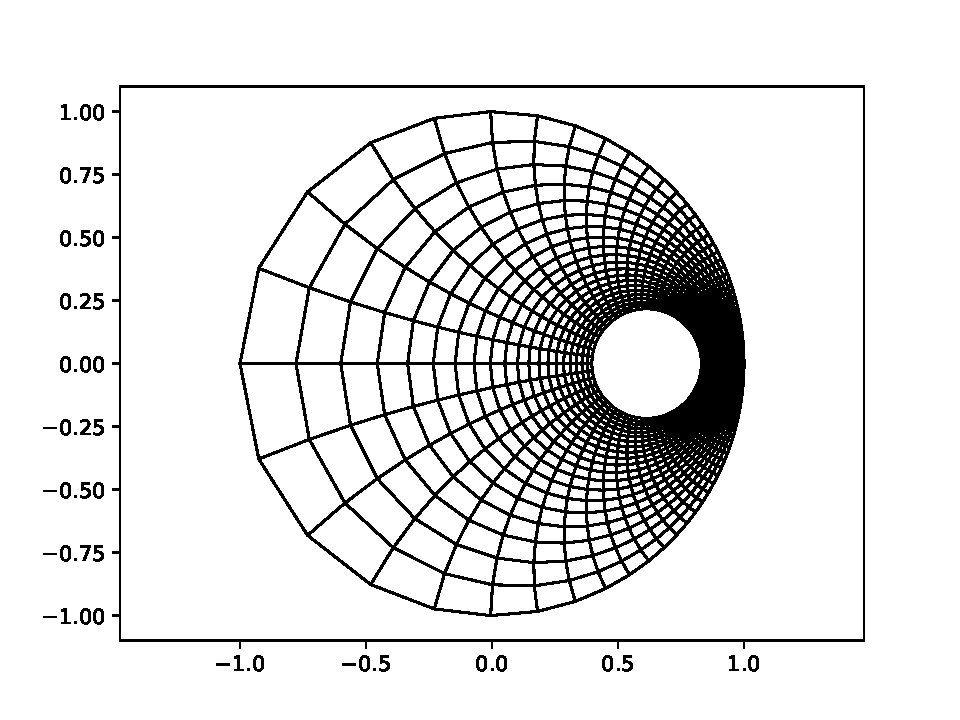
\includegraphics[width=0.8\linewidth]{conformal.pdf}
    \caption{conformal mapping from $0\leq x\leq 1, 0\leq y\leq 2\pi$ by function $\omega(z)$ in \eqref{eq:conf}}
    \label{fig:conformal}
\end{figure}

It is known that a line constant in $\xi$ will map to a circle. Further, $(\xi, \eta=0)$ is the points on the real axis to the left of the centres, while $(\xi, \eta=\pi)$ is the real points to the right of the centres. The centre is then the average of these.
\begin{align*}
    c(\xi) =  & \frac{\omega(\xi, 0) + \omega(\xi, \pi)}{2}
    \\
    2c(\xi) = & \frac{2e^{\xi}e^0-3}{3e^{\xi}e^0 - 2} + \frac{2e^{\xi}e^{i\pi} - 3}{3e^{\xi}e^{i\pi} -2} = \frac{2e^{\xi}-3}{3e^{\xi} - 2} + \frac{2e^{\xi}+ 3}{3e^{\xi}+2}
    \\
    =         & \frac{(2e^{\xi}-3)(3e^{\xi}+2) + (2e^{\xi}+3)(3e^{\xi}-2)}{(3e^{\xi}-2)(3e^{\xi}+2)}
    \\
    =         & \frac{12(e^{2\xi}-1)}{9e^{2\xi}-4}
    \\
    c(\xi) =  & \frac{6(e^{2\xi}-1)}{9e^{2\xi}-4}
\end{align*}

The radius of the circles can be found in a similar way.
\begin{align*}
    r(\xi) = & \omega(\xi, \pi) - c(\xi)
    \\
    =        & \frac{2e^{xi}+3}{3e^{\xi}+2} - \frac{6(e^{2\xi}-1)}{9e^{2\xi}-4}
    \\
    =        & \frac{5e^{\xi}}{9e^{2\xi}-4}
\end{align*}

With these functions, the top point as a function of the centre of the circle can be added to the plot in Figure \ref{fig:conformal}. This is done in Figure \ref{fig:cr}, for $0\leq \xi \leq 2\pi$, and $\pm r(\xi)$.

\begin{figure}
    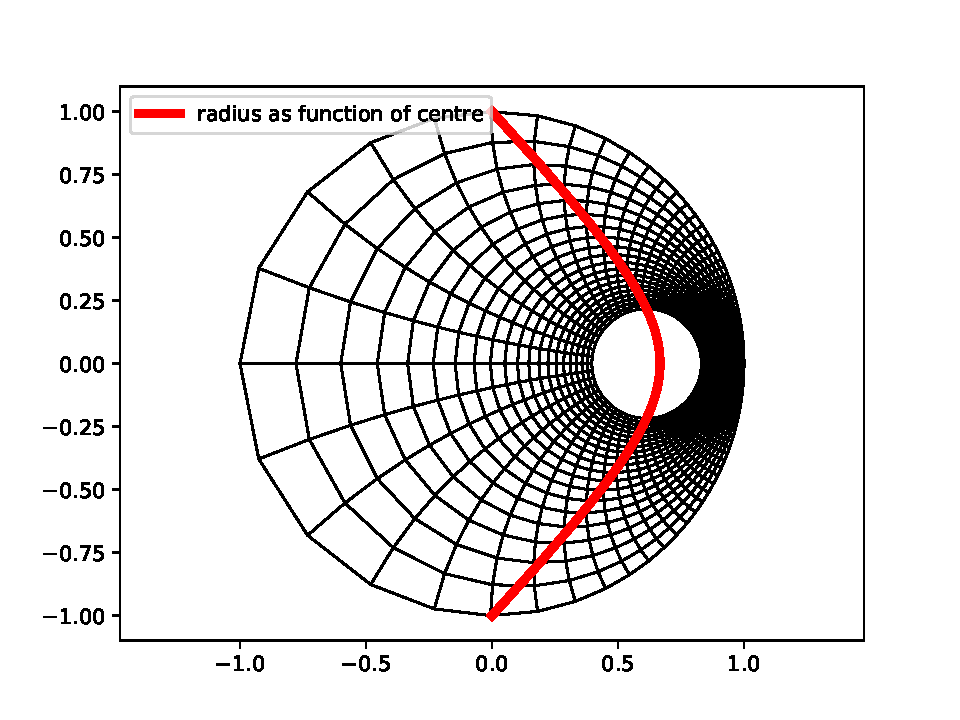
\includegraphics[width=0.8\linewidth]{conformal_cr.pdf}
    \caption{The conformal mapping of $\omega(z)$, along with the top-point of the circles, as function of the centre.}
    \label{fig:cr}
\end{figure}


\section*{Problem 4}
Followng the step-by-step instructions, I wrote a mesh-generator which used Delaunay to triangulate any polygon.

\subsection*{b}
The boundary points are added by linear interpolation between each corner.

\subsection*{d}
To determine if a triangle is outside the polygon, I make a test-point inside each triangle $abc$ by $p_{test} = a + 0.5ab + 0.25 bc$, and then the \texttt{inpolygon}-function.

\subsection*{e}
The area and circumcentre are calculated with formula from Wikipedia. This is repeated until no triangle is too large

\subsection*{h}
The triangulation is refined by adding the centre point of each edge.


The final triangulated mesh for the parameters specified is shown in Figure \ref{fig:triang}. It shares a great resembelance to the one in Figure (h) in the problem description.

\begin{figure}
    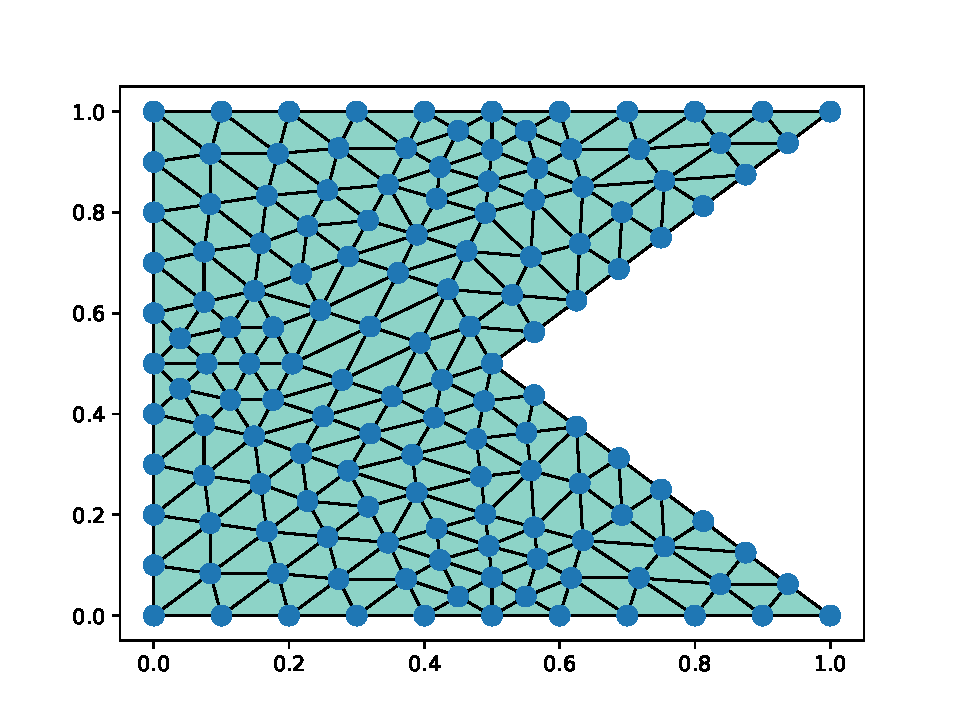
\includegraphics[width=0.8\linewidth]{triangulated.pdf}
    \caption{The triangulated mesh with specified parameters.}
    \label{fig:triang}
\end{figure}



\begin{thebibliography}{99}
\end{thebibliography}

\end{document}

